Perancangan sistem merupakan tahap penting dalam pengembangan perangkat lunak karena menjadi dasar bagi implementasi yang terarah. Pada tahap ini, dilakukan perancangan Generator Konten \textit{website} berbasis API untuk menyediakan solusi pengelolaan templat \textit{website} dan sinkronisasi data. Perancangan ini bertujuan untuk mendukung interoperabilitas, keamanan, dan keandalan sistem, serta menjadi pedoman teknis dalam proses implementasi berikutnya.

Arsitektur Generator Konten \textit{website} berbasis API terdiri dari enam komponen utama yang dapat dilihat pada Gambar \ref{fig:ArsitekturGeneratorKontenWebsite}, berikut adalah penjelasan setiap komponen:
\begin{enumerate}[label=\alph*.]
            
    \item \textbf{API Generator Konten \textit{website}}\\ 
        API Generator Konten \textit{website} merupakan inti dari sistem ini. Komponen ini bertanggung jawab untuk menangani berbagai operasi yang berkaitan dengan templat \textit{website} dan proses \textit{generate \textit{website}} berdasarkan permintaan pengguna.\\

        Berikut adalah spesifikasi teknis API Generator Konten \textit{website}:
        \begin{enumerate}[label=\arabic*.]
                
            \item \textbf{Arsitektur:} Representational State Transfer (REST)
                    
            \item \textbf{Teknologi:} Bahasa pemrograman Javascript dengan \textit{runtime Node.js} dan \textit{framework Express.js}
                        
            \item \textbf{Pendekatan Desain:} Modular
                    
        \end{enumerate}

    \item \textbf{API Aplikasi Internal}\\
        API Aplikasi Internal berfungsi sebagai penghubung antara sistem generator dan aplikasi lain di lingkungan internal. Komponen ini menyediakan layanan untuk pengambilan dan pemuatan data.\\
                
        Berikut adalah spesifikasi teknis API Aplikasi Internal:
        \begin{enumerate}[label=\arabic*.]
                
            \item \textbf{Arsitektur:} \textit{Representational State Transfer} (REST)
                    
            \item \textbf{Teknologi:} Bahasa pemrograman Javascript dengan \textit{runtime Node.js} dan \textit{framework Express.js}
                        
            \item \textbf{Pendekatan Desain:} Fokus pada \textit{endpoint} untuk pengambilan data (GET) dan pemuatan data (POST)
                    
        \end{enumerate}
            
    \item \textbf{Modul Sinkronisasi Data}\\
        Modul Sinkronisasi Data adalah komponen yang bertugas memastikan bahwa data yang ada di aplikasi internal selalu \textit{up-to-date} dengan data terbaru dari basis data aplikasi web.

        Berikut adalah fungsi utama dari Modul Sinkronisasi Data:
        \begin{enumerate}[label=\arabic*.]
                
            \item \textbf{Sinkronisasi Terjadwal:} Penjadwalan berbasis \textit{event-driven} menggunakan library \texttt{node-schedule}.
                    
            \item \textbf{Ekstraksi Data:} Mengambil data dari basis data aplikasi web berdasarkan konfigurasi yang ada dibasis data templat.
                    
            \item \textbf{Transformasi Data:} Melakukan validasi dan modifikasi pada data hasil ekstraksi agar sesuai dengan format yang diterima oleh API Aplikasi Internal.
                    
            \item \textbf{Load Data:} Mengirim data ke API Aplikasi Internal.
            \end{enumerate}

        Proses sinkronisasi data terdiri dari langkah-langkah berikut:
        \begin{enumerate}[label=\arabic*.]
            \item Modul membaca jadwal sinkronisasi dari entitas \textit{job}.
            \item Modul mengakses konfigurasi koneksi basis data dari entitas \textit{db\_config}.
            \item Modul melakukan ekstraksi data dari tabel yang ditentukan di basis data aplikasi web.
            \item Data yang diekstrak divalidasi dan dimodifikasi agar sesuai dengan struktur data yang dibutuhkan oleh API tujuan berdasarkan aturan yang sudah didefinisikan di entitas \textit{job}.
            \item Data yang telah diproses dikirim ke API Aplikasi Internal menggunakan metode \texttt{POST}.
        \end{enumerate}
        
    \item \textbf{Basis Data Templat}\\ 
        Basis Data Templat adalah pusat penyimpanan templat \textit{website} dan informasi tambahan yang terkait. Basis data ini dirancang menggunakan \textit{Relational Database Management System} (RDBMS) PostgreSQL.

    \item \textbf{Basis Data Aplikasi Web}\\
        Basis Data Aplikasi Web digunakan untuk menyimpan data dari aplikasi web yang dihasilkan oleh Generator Konten \textit{website}. Basis data ini dirancang menggunakan \textit{Relational Database Management System} (RDBMS), seperti PostgreSQL atau MySQL, tergantung pada kebutuhan proyek.

    \item \textbf{Pengguna}\\
        Pengguna adalah entitas yang berinteraksi dengan API Generator Konten \textit{website} melalui \textit{endpoint} yang disediakan. Mereka dapat mengelola templat, meminta generasi \textit{website}, serta memantau status proses melalui antarmuka yang tersedia.
            
\end{enumerate}

\begin{figure}[H]
    \centering
    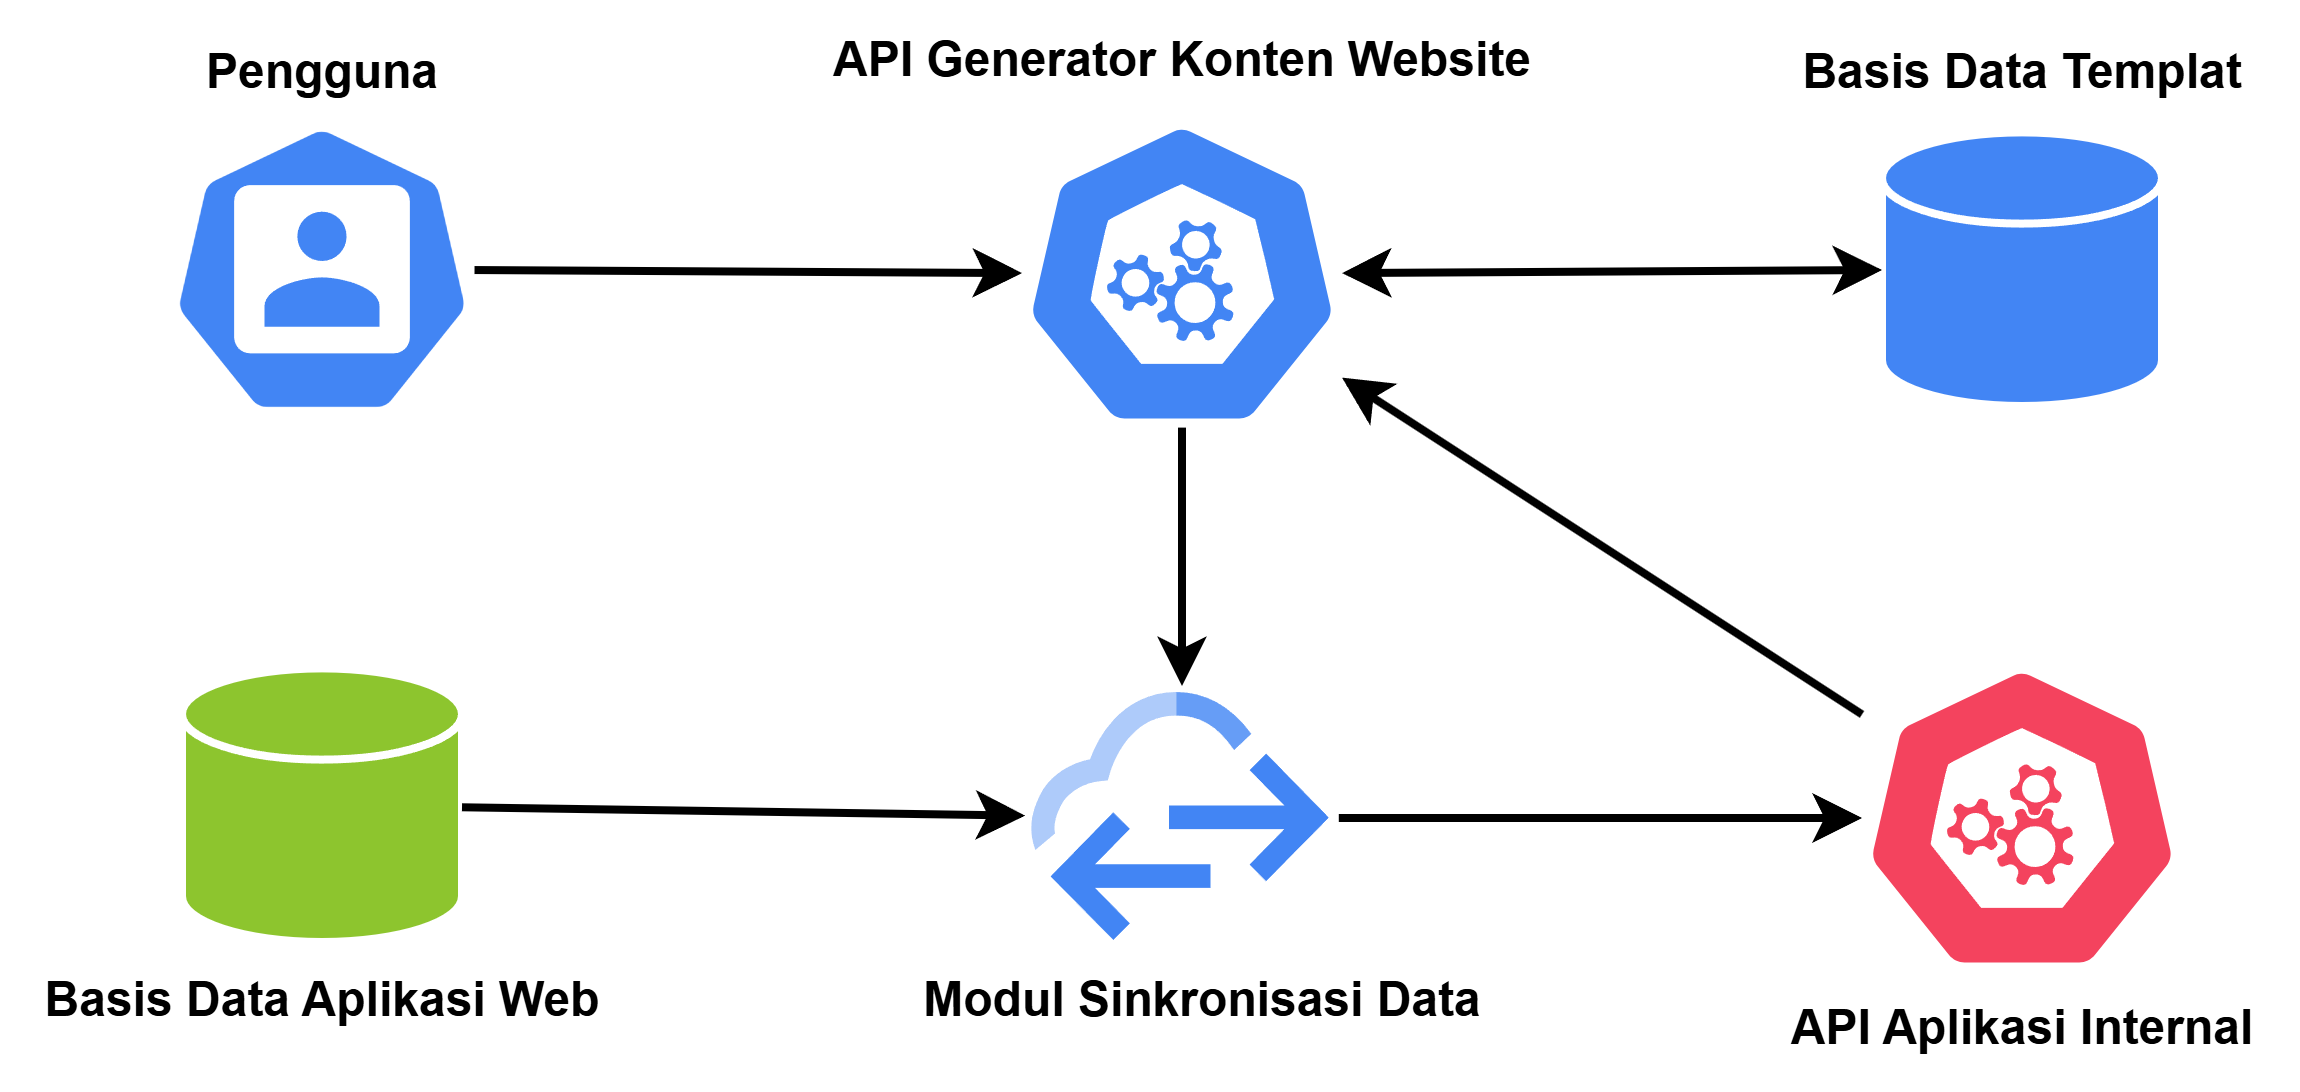
\includegraphics[width=0.8\linewidth]{figures/ArsitekturGeneratorKontenWebsite.png}
    \caption{Arsitektur Generator Konten \textit{website}}
    \label{fig:ArsitekturGeneratorKontenWebsite}
\end{figure}
